% Created 2018-09-26 Wed 21:07
% Intended LaTeX compiler: pdflatex
\documentclass[journal=ancac3,manuscript=article,email=true,hyperref=true,keywords=false]{achemso}
\usepackage[utf8]{inputenc}
\usepackage{graphicx}
\usepackage{float}
\usepackage{xcolor}
\usepackage{amsmath}
\usepackage{amssymb}
\usepackage{lineno}
\usepackage{todonotes}
\usepackage{times}

\author{Tian Tian}
\affiliation{Institute for Chemical and Bioengineering, ETH Z{\"{u}}rich,  Vladimir Prelog Weg 1, CH-8093 Z{\"{u}}rich, Switzerland}
\altaffiliation{T. T. and D. S. contributed equally to this work}
\author{Declan Scullion}
\affiliation{School of Mathematics and Physics, Queen's University Belfast, BT7 1NN, United Kingdom}
\altaffiliation{T. T. and D. S. contributed equally to this work}
\author{Dale Hughes}
\affiliation{School of Mathematics and Physics, Queen's University Belfast, BT7 1NN, United Kingdom}
\author{Lu Hua Li}
\affiliation{Institute for Frontier Materials, Deakin University, Waurn Ponds, Victoria, Australia}
\author{Chih-Jen Shih}
\affiliation{Institute for Chemical and Bioengineering, ETH Z{\"{u}}rich,  Vladimir Prelog Weg 1, CH-8093 Z{\"{u}}rich, Switzerland}
\author{Jonathan Coleman}
\affiliation{School of Physics, Centre for Research on Adaptive Nanostructures and Nanodevices (CRANN) and Advanced Materials and BioEngineering Research (AMBER), Trinity College Dublin, Dublin 2, Ireland.}
\author{Manish Chhowalla}
% \affiliation{Materials Science and Engineering, Rutgers University, 607 Taylor Road, Piscataway, New Jersey 08854, USA.}
\affiliation{Department of Materials Science \& Metallurgy, University of Cambridge, CB3 0FS, United Kindom}
\author{Elton J. G. Santos}
\email{e.santos@qub.ac.uk}
\affiliation{School of Mathematics and Physics, Queen's University Belfast, BT7 1NN, United Kingdom}
\date{}
\title{The Unified Nature of the Dielectric Properties of Two-Dimensional Materials}
% \title{Unified Understanding of the Dielectric Nature of Two-Dimensional Materials}
\begin{document}

\newpage{}


% \section{Introduction}
% \label{sec:org2ea169d}
% \linenumbers{}

{\bfseries Dielectric constant, which defines the polarization of the
  media, is a key quantity in condensed matter. Here we show that
  despite its fundamental transcendence, the dielectric constant does
  not define unequivocally the dielectric properties of a
  two-dimensional (2D) material. We found instead that the dielectric
  polarizability correctly captures the dielectric nature of a 2D
  material which is strongly dependent on the long-range
  electron-electron interaction.  We reveal a long-sought universal
  framework where electronic, geometrical and dielectric properties
  are intrinsically correlated through the polarizability opening the
  door to probe quantities yet not directly measurable, e.g. thickness
  of an atom.  By using this framework, we unify the concept of
  dielectric properties in any material dimension through a dielectric
  anisotropy index which defines the degree of controllability of the
  dielectric features of a compound. A universal boundary line
  separates the 3D and 2D behaviors where materials likely to have
  similar properties as layered materials collapsed onto.  }

The central place of dielectric properties, especially the static
dielectric constant in material research
\cite{Dressel_2001_electrodynamics} drives the pursuit for a unified
model between the electronic and dielectric properties of materials.
% In fact, some pioneering work\cite{Moss_1950_relation} discovered
% relations between the dielectric constant $\varepsilon$ and other
% physical properties, in particular the band gap $E_{\mathrm{g}}$ of
% bulk semiconductors.
In fact, some pioneer
work\cite{Moss_1950_relation,Moss_1985_n_Eg,Ravindra_1979_eps_Eg,Ravindra_2007_Eg_rev}
proposed the empirical model between the energy bandgap
$E_{\mathrm{g}}$ and dielectric constant $\varepsilon$ of bulk
semiconductors, such as the famous Moss relation
\cite{Moss_1950_relation,Moss_1985_n_Eg}:
\begin{equation}
\label{eq:Moss-relations}
\varepsilon^{2} E_{\mathrm{g}} \approx 95\ \mathrm{eV}
\end{equation}
Despite the minor difference between the empirical formulae proposed,
such general relation  is of high
practical importance for material design and engineering: with the
Moss relationship or other similar models, it is feasible to predict
the dielectric constant (and hence other parameters such as refractive
index, Bohr radius, exciton binding energy, etc.) of a bulk material
from the its bandgap with with a reasonable degree of certainty
% The
% existence of such general relationship is also of high practical
% importance: it is generally more straightforward and accurate to
% measure the band gap $E_{\mathrm{g}}$ than the static dielectric
% constant $\varepsilon$ of a bulk material, as the latter is strongly
% dependent on several critical details on the sample measurements, such
% as contamination, disorder, and model interpretation.
While the electronic-dielectric relation for bulk semiconductors is
well-established, it is unknown if such equation still exists in
atomically-thin two-dimensional (2D) materials \cite{Novoselov_2016},
due to (i) the dielectric screening of a 2D material is attenuated and
anisotropic
\cite{Keldysh_1979_eps_multi,Sharma_1985,Low_2014_screening_BP,Cudazzo_2011_screening_2D,Bechstedt_2012}
and (ii) the static dielectric constant, a quantity associated with
the macroscopic dielectric and optoelectronic properties and commonly
obtained by theoretical calculations of 2D materials
\cite{Ramasubramaniam_2012,Wang_2016_Aip,Laturia_2018}, may not well
describe this microscopic and anisotropic dielectric nature of 2D
materials \cite{Cudazzo_2010_screen2D,Cudazzo_2011_screening_2D}.
% Therefore, an
% accurate description of the 2D dielectric nature is the prerequisite
% for a 2D Moss-like relation, which could be used to make predictions
% for less-investigated layered crystals and to create materials design
% rules at an accurate level.
Here we show that instead of the dielectric constant $\varepsilon$,
the 2D polarizabilty $\alpha$ correctly captures the dielectric nature
of a 2D material. Based on both theoretical model and first principle
calculations, we reveal the long-sought universal dielectric scaling
relations for 2D materials, depend both on the electronic and
structural information: the in-plane polarizability
$\alpha^{\parallel}$ is inversely proportional to the minimal bandgap
$E_{\mathrm{g}}$, while the out-of-plane polarizability
$\alpha^{\perp}$ is directly related with the thickness
$\delta$ of a 2D materials. We further introduce the concept of
dielectric anisotropy index, to unify 2D and 3D dielectric
property. The proposed universal dielectric scaling relationships of
2D compounds introduce a general pathway for the exploration of their
complex physical and chemical phenomena well beyond the currently
possible applications.
% Based on this
% framework, we further unify the concept of dielectric properties of
% any material dimension, by the dielectric anisotropy index, 
% An analytical quantum-mechanical model is developed
% which give a sound background to the dielectric-scale
% relationships.
% Using such unified relations unify the dielectric
% properties between the 2D materials and their 3D counterparts in a
% natural manner, which ultimately pushes the boundary of the
% understanding of electronic screening in both dimensions.
% The discovery of scaling relationships between dielectric and electronic
% and structural properties in 2D compounds introduces a new and general
% pathway for the exploration of their complex physical and chemical
% phenomena well beyond the currently possible applications.

% \section{Results}
% \label{sec:org752ca78}

\subsection{Dielectric Nature of 2D Materials}
\label{sec:2d}

In pursuit of the Moss-like relation for 2D materials, an accurate
description of their dielectric properties needs to be established,
since the concept of macroscopic dielectric constant is ill-defined
for 2D materials
\cite{Cudazzo_2010_screen2D,Cudazzo_2011_screening_2D,Nazarov_2015_2D_3D}. As
shown in Figure \ref{fig-1}a, in routine first principles
calculations, an isolated 2D material is placed in the xy-plane of a
periodically repeating superlattice (SL) with a length $L$ along the
z-direction separating the cell images. The macroscopic dielectric
tensor from the superlattice $\varepsilon_{\mathrm{SL}}^{pq}$, is
determined through fundamental electrostatics by the response of the
polarization density $\boldsymbol{P}^{p}$ under small perturbative
external field $\boldsymbol{E}^{q}$, where $p$, $q$ are the directions
of polarization and electric field,
respectively\cite{Dressel_2001_electrodynamics}:
\begin{subequations}
  \begin{eqnarray}
      \label{eq:def-eps-1}
    &\varepsilon^{pq} &= \kappa^{pq} +
                                 {\displaystyle \frac{\partial \boldsymbol{P}^{p}}
                                 {\varepsilon_{0} \partial \boldsymbol{E}^{q}}} \\
          \label{eq:def-eps-2}
    &\boldsymbol{P}^{p} &=  {\displaystyle \frac{\boldsymbol{u}^{p}}{\Omega}}
                          = {\displaystyle \frac{{\displaystyle
          \int_{\mathrm{SL}} \rho(\boldsymbol{r}) \boldsymbol{r}^{p} d^{3}\boldsymbol{r}}}
                          {AL}}
  \end{eqnarray}
\end{subequations}
where $\kappa$ is the dielectric tensor of the environment,
$\boldsymbol{u} = {\displaystyle \int_{\mathrm{SL}}
  \rho(\boldsymbol{r}) \boldsymbol{r}^{p} d^{3}\boldsymbol{r}}$ is the
total dipole moments of the SL, $\rho$ is the spatial charge density,
$\Omega=AL$ is the volume, $A$ is the xy-plane area of the SL and
$\varepsilon_{0}$ is vacuum permittivity. For the majority of 2D
semiconductors, the off-diagonal elements of the dielectric tensor
($p \neq q$) tend to be negligible.  Considering that the 2D material
is placed in vacuum ($\kappa^{pp} = 1$ and $\kappa^{pq} = 0$), we can
distinguish two components, namely the in-plane
($\varepsilon_{\mathrm{SL}}^{\parallel}$) and out-of-plane
($\varepsilon_{\mathrm{SL}}^{\perp}$) dielectric constants, where
$\varepsilon_{\mathrm{SL}}^{\parallel} =
(\varepsilon_{\mathrm{SL}}^{xx} + \varepsilon_{\mathrm{SL}}^{yy})/2$
and
$\varepsilon_{\mathrm{SL}}^{\perp} =
\varepsilon_{\mathrm{SL}}^{zz}$. The absense of bonding perpendicular
to the 2D plane confines the induced dipoles along the
\textit{z}-direction: as shown in Figure \ref{fig-1}a and
Supplementary Figure SXX \todo{check}, the charge density difference
between zero and finite electric fields,
$\Delta \rho=\rho(\boldsymbol{E}) - \rho(\boldsymbol{E}=0)$ along the
z-axis for an isolated 2H-MoS$_{2}$ layer under
$|\boldsymbol{E}_{z}|=0.01 \mathrm{V\cdot \AA}^{-1}$ only extends to
$\sim{}$12 \AA{} along the z-direction. When $L$ is large enough that
the induced dipoles from periodic images do not interact,
$\boldsymbol{u}$ equals the total dipole moments of a monolayer 2D
materials and independent of the SL size. As a consequence, we can see
from Eqs. \ref{eq:def-eps-1} and \ref{eq:def-eps-2}, that both
$\varepsilon^{\parallel}_{\mathrm{SL}}$ and
$\varepsilon^{\perp}_{\mathrm{SL}}$ depend on $L$. We show this by
plotting $\varepsilon^{\parallel}_{\mathrm{SL}}$ and
$\varepsilon^{\perp}_{\mathrm{SL}}$ calculated from density functional
theory (DFT) as functions of $L$ for P$\bar{6}$m2 (2H) transitional
metal dichalcogenides (TMDCs, 2H-MX$_{2}$, where M=Mo, W and X=S, Se,
Te), in the top panels of Figure \ref{fig-1}b and \ref{fig-1}c,
respectively.
% We observe that neither
% $\varepsilon^{\parallel}_{\mathrm{SL}}$ nor
% $\varepsilon^{\perp}_{\mathrm{SL}}$ converges with $L$ due to fact
% that the long-range Coulomb interaction could not be completed
% screened within the range of magnitudes computationally accessible
% \cite{Hueser_2013_2Dvs3D}.
As a result, the $L$-dependency of $\varepsilon_{\mathrm{SL}}$ makes
it impractical to represent the dielectric nature of a 2D material
both theoretically and experimentally, because the size of vacuum
layer must always be considered. To solve this problem, we need to
find the $L$-independent alternative of
$\varepsilon_{\mathrm{SL}}$. As described before, by multiplying
Eq. \ref{eq:def-eps-2} with $L$ we get the sheet polarization density
of a 2D material $\boldsymbol{\mu}_{\mathrm{2D}}$, such that
$\boldsymbol{\mu}_{\mathrm{2D}}^{p} = \boldsymbol{P}^{p}L =
\boldsymbol{u}^{p}/A$, which is dependent with $L$ due to the invariablity
of $\boldsymbol{u}$ and $A$. Similar to the definition of molecular
polarizability \cite{Israelachvili_2011},
$\boldsymbol{\mu}_{\mathrm{2D}}$ is associated with the 2D
polarizability $\alpha_{\mathrm{2D}}$ through:
$\boldsymbol{\mu}^{p} = \sum_{q} \alpha_{\mathrm{2D}}^{pq}
\boldsymbol{E}_{\mathrm{loc}}^{q}$ \cite{T_bik_2004}, where
$\boldsymbol{E}_{\mathrm{loc}}$ is the local electric field. In the
in-plane direction, the continuity of electric field gives
$\boldsymbol{E}^{\parallel}_{\mathrm{loc}}=\boldsymbol{E}^{\parallel}$
\cite{Markel_2016}. Perpendicular to the 2D plane, the dipole
screening yields
$\boldsymbol{E}_{\mathrm{loc}}^{\perp}=\boldsymbol{E}^{\perp}+\boldsymbol{\mu}_{\mathrm{2D}}^{\perp}/L$
\cite{Meyer_2001_dipole_slab,T_bik_2004}. Combining with
Eqs. \ref{eq:def-eps-1} and \ref{eq:def-eps-2}, we derive the
expressions for the in-plane and out-of-plane 2D polarizabilities,
$\alpha_{\mathrm{2D}}^{\parallel}$ and $\alpha_{\mathrm{2D}}^{\perp}$, respectively:
\begin{subequations}
\begin{eqnarray}
  \label{eq:alpha-para-def}
  &\alpha_{\mathrm{2D}}^{\parallel} &= \varepsilon_{0}(\varepsilon_{\mathrm{SL}}^{\parallel} - 1)L\\
  \label{eq:alpha-perp-def}
  &\alpha_{\mathrm{2D}}^{\perp} &= \varepsilon_{0}\left(1 - {\displaystyle \frac{1}{\varepsilon_{\mathrm{SL}}^{\perp}}}\right)L
\end{eqnarray}
\end{subequations}
The bottom panels of Figure \ref{fig-1}b and \ref{fig-1}c show the
$\alpha_{\mathrm{2D}}^{\parallel}$ and $\alpha_{\mathrm{2D}}^{\perp}$
of the TMDCs as functions of $L$, calculated using
Eqs. \ref{eq:alpha-para-def} and \ref{eq:alpha-perp-def}. We observe
that both $\alpha_{\mathrm{2D}}^{\parallel}$ and
$\alpha_{\mathrm{2D}}^{\perp}$ remain almost constant when $L>$15
\AA{}. In addition, as shown Figure \ref{fig-1}d and \ref{fig-1}e,
respectivel, the model-predicted
$\varepsilon_{\mathrm{SL}}^{\parallel}-L$ and
$\varepsilon_{\mathrm{SL}}^{\perp}-L$ relations from Eqs.
\ref{eq:alpha-para-def} and \ref{eq:alpha-perp-def} nicely reproduce
the trends from Figures \ref{fig-1}b and \ref{fig-1}c. These findings
indicate that the 2D polarizability, instead of the dielectric
constant, is the true descriptor of the dielectric properties of 2D
materials. More discussion about the choice of the 2D polarizability
and comparison with other methods can be find in Supplementary Section
SXX \todo{xxx}.


% It is also worth mentioning that the dielectric properties of 2D
% materials are also often modeled using an effective medium approach,
% which treats the 2D material as a slab with effective permittivity
% $\varepsilon_{\mathrm{2D}}$ and thickness $\delta$
% \cite{Sharma_1985,Cudazzo_2011_screening_2D,Matthes_2016,Trolle_2017_eps_subst,Laturia_2018}. Such
% methods require \textit{a priori} determination of $\delta$, a
% quantity with controversial definitions \cite{Mas_Ballest__2011}. In
% such approaches, $\varepsilon_{\mathrm{2D}}$ and $\delta$ have to be
% determined by fitting the $L$-dependent data of
% $\varepsilon_{\mathrm{SL}}$, which is not only computational
% expensive, but also fails to capture the anisotropy of the 2D
% dielectric properties (see Supplementary Section S1). On the other
% hand, calculating 2D polarizabilities requires no knowledge of
% $\delta$ (see Eqs. \ref{eq:alpha-para-def} and
% \ref{eq:alpha-perp-def}), and correctly presents the anisotropy of 2D
% dielectric nature that $\alpha^{\parallel} > \alpha^{\perp}$.  With
% the polarizability as the true descriptor of 2D dielectric properties,
% we will reveal the universal Moss-like relation of 2D materials from
% both theoretical and first principles studies.

\iffalse
\subsection{Polarizability-Based Theoretical Model}
\todo[inline]{In case of Nat. Nanotechnol., I would like to move all
  theoretical information to SI}.
Based on the 2D polarizability, we
then theoretically investigate the potential existence of the
Moss-like relations for 2D materials.  Due to its highly anisotropic
nature, the wavefunction of an isolated 2D material $\psi(\mathbf{r})$
can be separated into the in- and out-of-plane components, similar to
the treatment of quantum wells (QW),\cite{davies_physics_1997} such
that $\psi^{\parallel}(\boldsymbol{\rho})$ and $\psi^{\perp}(z)$, such
that $\psi=\psi^{\parallel}\psi^{\perp}$, where
$\boldsymbol{\rho}=(x, y)$ is the in-plane coordinate. Using the Bloch
theorem, the periodic $\psi^{\parallel}(\boldsymbol{\rho})$ can be
further expressed as
$\psi^{\parallel}(\boldsymbol{\rho})=e^{i\mathbf{k} \cdot
  \boldsymbol{\rho}}u(\boldsymbol{\rho})$, where $\mathbf{k}$ is the
in-plane wave vector and $u(\boldsymbol{\rho})$ is periodic function
in the xy-plane. According to the random phase approximation (RPA)
theory\cite{Adler_1962}, $\varepsilon_{\mathrm{SL}}$ is the
$\mathbf{q} \to 0$ and $\omega \to 0$ limits of the non-interacting
dielectric function $\varepsilon(\mathbf{q}, \omega)$, where
$\mathbf{q}$ is the momentum transfer and $\omega$ is the frequency:
\begin{equation}
  \label{eq:RPA-eps2}
  \varepsilon_{\mathrm{SL}}
  = \lim_{\mathbf{q} \to 0} 1 + \frac{2e^{2}}{\varepsilon_{0} |\mathbf{q}|^{2} \Omega}
  \sum_{\mathrm{k, c, v}}
  \frac{|<\psi_{\mathrm{v}}(\mathbf{k})|e^{-i\mathbf{q}\mathbf{r}}|\psi_{\mathrm{c}}(\mathbf{k+q})>|^{2}}
  {E_{\mathrm{c}}(\mathbf{k+q}) - E_{\mathrm{v}}(\mathbf{k})}
  \left[f(\psi_{\mathrm{c}}) - f(\psi_{\mathrm{v}})\right]
\end{equation}
where $e$ is the unit charge, c, v are the conduction and valence
bands, $E$ is the eigenenergy of individual bands, and $f$ is the
Fermi-Dirac distribution function. Taking the limit that $L\to\infty$,
when $\varepsilon^{\perp}_{\mathrm{SL}} \approx 1$, we have
$1-1/\varepsilon^{\perp}_{\mathrm{SL}} \approx
(\varepsilon_{\mathrm{SL}}^{\perp} - 1)$. Combine this with
Eqs. \ref{eq:alpha-para-def}, \ref{eq:alpha-perp-def} and
\ref{eq:RPA-eps2}, and taking the difference between the properties of
in-plane and out-of-plane polarizabilities, we derive the expressions
for $\alpha^{\parallel}$ and $\alpha^{\perp}$ under small perturbation
(details see Supplementary Section S4):
\begin{subequations}
  \begin{eqnarray}
  \label{eq:alpha_para_RPA}
  & \alpha^{\parallel} &= \frac{2e^{2}}
  {(2 \pi)^{2}} \int d^{2}\mathbf{k} \sum_{\mathrm{c, v}}
  \frac{|<u_{\mathrm{v}}(\mathbf{k})|\nabla|u_{\mathrm{v}}(\mathbf{k})>|^{2}}
                         {E_{\mathrm{c}}(\mathbf{k}) - E_{\mathrm{v}}(\mathbf{k})} \\
  \label{eq:alpha_perp_RPA}
  & \alpha^{\perp} &= \frac{2e^{2}}{(2 \pi) ^{2}} \int d^{2}\mathbf{k}
  \sum_{\mathrm{c, v}}
  \frac{|<\psi_{\mathrm{v}}(\mathbf{k})|z|\psi_{\mathrm{c}}(\mathbf{k})>|^{2}}
  {E_{\mathrm{c}}(\mathbf{k}) - E_{\mathrm{v}}(\mathbf{k})}
  \end{eqnarray}
\end{subequations}
where the integral is performed within the first Brillouin Zone (BZ)
in the reciprocal $\mathbf{k}$-plane. Although they only differ by the
numerator inside the integral, the distinct behaviors of $u(\rho)$
(periodic function) and $\psi(z)$ (confined to the 2D material) give
rise to the different relations of $\alpha^{\parallel}$ and
$\alpha^{\perp}$. Using the $\mathbf{k} \cdot \mathbf{p}$ theory,
Eq. \ref{eq:alpha_para_RPA} is evaluated to be
$\alpha^{\parallel} = N e^{2}/(2\pi E_{\mathrm{g}})$, where $N$ is the
degeneracy associated with the minimal bandgap
\cite{Jiang_2017_Eg_Eb}. On the contrary, $\psi(z)$ is the solution to
the Schr\"{o}dinger equation with Hamiltonian
$\mathcal{H} = -\hbar^{2} \nabla^{2}/2m_{e} + V(z)$, where $\hbar$ is
the reduced Planck constant, $m_{e}$ is electron mass and $V(z)$ is
the confined Coulombic potential along the z-direction created by the
nuclei \cite{davies_physics_1997,ihn_semiconductor_2009}. Using a
simple particle-in-box model, we show that both the numerator and
denominator parts of Eq. \ref{eq:alpha_perp_RPA} are independent of
$E_{g}$ but instead modulated by the size of the potential confinement
(details see Supplementary Section S4). We further prove, using both
quantum mechanical and fundamental electrostatic models, that
$\alpha^{\perp}$ is actually proportional to the size of potential
confinement (details see Supplementary Section S4), which we may
relate with the thickness $\delta$ of the 2D material. Now we may
finally propose the 2D analog of the Moss relation with both in- and
out-of-plane polarizations:
\begin{subequations}
\begin{eqnarray}
\label{eq:2D-Moss-para}
  &\alpha^{\parallel} &\propto E_{g}^{-1} \\
  \label{eq:2D-Moss-perp}
  &\alpha^{\perp} & \propto \delta
\end{eqnarray}
\end{subequations}
which form the main conclusion of this work. Next, we will validate
the proposed 2D Moss-like relations using first principle
calculations.
\fi


\subsection{2D Moss Relations Based on 2D Polarizabilities}
\label{sec:first-principles}
We study several types of 2D materials of different electronic and
optical properties as show in Figure \ref{fig-2}, including transition
metal dichalcogenides (TMDCs, with the formula MX\(_{\text{2}}\),
where M is a metal in group 4, 6, 10 and X=O, S, Se, Te), metal
monochalcogenides (Ga$_{2}$S$_{2}$, Ga$_{2}$Se$_{2}$), cadmium halides
(CdX$_2$, X=Cl, I), hexagonal boron nitride (BN), graphene derivatives
(fluorographene (C$_{2}$F$_{2}$), graphane (C$_{2}$H$_{2}$)),
phosphorene (P$_{4}$) and thin layer organic-inorganic perovskites
(ABX$_{3}$).  For the TMDCs, we consider 2 lattice phases, namely the
2H (P\(\bar{6}\)m2 space group) and 1T (P3m1 space group).  The static
2D polarizabilities are calculated from the static dielectric response
of the selected 2D materials using density functional theory (DFT)
with the Heyd-Scuseria-Ernzerhof hybrid functionals (HSE06) using the
Vienna Ab Initio Simulation Package (VASP) including spin-orbit
coupling to avoid limitations on the description of band gaps and
dielectric functions (see Methods for details).

Figure \ref{fig-3}a shows the calculated bandgap $E_{\mathrm{g}}$
(blue dots) and polarizabilities (bar plots) of all the 2D materials
investigated, covering a wide spectrum range from far infrared to
ultraviolet. Note from dimension analysis, it is more intuitive to
express the polarizability as $\alpha/(4 \pi \varepsilon_{0})$, which
has unit of \AA. We find that $\alpha^{\parallel}$ has a general
descending trend when $E_{\mathrm{g}}$ increases. On the other hand,
no apparent trend between $\alpha^{\perp}$ and $E_{\mathrm{g}}$ is
observed (see Supplementary Section S2.2), which appears to be in good
agreement with our polarizability-based theoretical model. We now
validate Eq. \ref{eq:2D-Moss-para} and \ref{eq:2D-Moss-perp} using the
polarizabilities calculated by first principle calculations. Figure
\ref{fig-3}b shows $(4 \pi \varepsilon_{0})/\alpha^{\parallel}$ (in
\AA{}) as a function of $E_{\mathrm{g}}$ (in eV) for the 2D materials
investiaged (circle dots), with a linear regression slope of ~0.182
and $R^{2}$ of 0.84. From Ref. \citenum{Jiang_2017_Eg_Eb}, the slope
between $(4 \pi \varepsilon_{0})/\alpha^{\parallel}$ and $E_{g}$ is
$8\pi^{2}\varepsilon_{0} \mathrm{\AA}/(eN) \approx 0.436/N$, which
yields $N$ betweem 2 and 3, which is reasonable for the 2D materials
studied. We observe that materials with lower $E_{\mathrm{g}}$ ($<$4
eV) generally lie close to the regression line, while the deviation
becomes greater for materials with $E_{\mathrm{g}}>$4 eV, which has
also been observed in the $E_{\mathrm{b}}-E_{\mathrm{g}}$ relation of
2D materials \cite{Olsen_2016_hydrogen,Jiang_2017_Eg_Eb}. We also
discover that the linearity between
$(4 \pi \varepsilon_{0})/\alpha^{\parallel}$ and $E_{\mathrm{g}}$ is
better when the bandgap is calculated using the HSE06 hybrid
functionals, compared with that from the Perdew--Burk--Ernzerhof (PBE)
exchange correlations (details see Supplementary Section S2 and
Supplementary Figure S5), which can be explained by the fact that the
electronic structure, in particular the bandgap, is generally better
predicted at HSE06 level than PBE level \cite{Heyd_2005}. It should be
noted that although even more accurate estimation of both
$\varepsilon$ and $E_{\mathrm{g}}$ can be achieved via many-body
Green’s function method (GW) together with the Bethe-Salpeter equation
(BSE), the convergence of such method is known to be highly affected
by the dielectric screening of 2D materials
\cite{Hueser_2013_2Dvs3D}. Combining the accuracy, computational
effort and convergence, the choice of the HSE06 hybrid functional may
be most suitable to present the true 2D Moss-like relationship between
$\alpha^{\parallel}$ and $E_{\mathrm{g}}$. 

We further examine the relation between $\alpha^{\perp}$ and the
thickness of a 2D material proposed in
Eq. \ref{eq:2D-Moss-perp}. Here we choose the ``covalent'' thickness
$\delta_{\mathrm{cov}}$ of a 2D material, which is defined as the
longest distance along the z-direction between any two atom nuclei
plus their covalent radii:
\begin{equation}
  \label{eq:cov-thick}
  \delta_{\mathrm{cov}} = \mathrm{max}(|z^{i} - z^{j}|
  + r^{i}_{\mathrm{cov}} + r^{j}_{\mathrm{cov}})
\end{equation}
where i, j are two atoms in the 2D material and $r_{\mathrm{cov}}^{i}$
is the covalent radius of atom i (Figure \ref{fig-3}c inset). As shown
in Figure \ref{fig-3}c, $\alpha^{\perp}/(4 \pi \varepsilon_{0})$
indeed shows an excellent linear correlation with
$\delta_{\mathrm{cov}}$, with $R^{2}=0.98$, and the slope very close
to $1/4\pi$. In addition to our theoretical predictions discussed
above, the perfect linear correlation between $\alpha^{\perp}$ and
$\delta_{\mathrm{cov}}$ has its strong physical meaning. Similar to
the molecular polarizability which characterizes the volume of
electron cloud of an isolated molecule \cite{Israelachvili_2011}, the
2D polarizability also characterizes the volume of the electron cloud
per unit area (from its definition), and naturally represents the
thickness of the electron cloud of the 2D material. The fact that the
thickness of the electron cloud can be approximated by the extension
of valence states in the z-direction, explains the close match between
the linear slope in Figure \ref{fig-3}c and $1/4\pi$ (see
Supplementary Section S4.1). In other words, the universal scaling
relation for $\alpha^{\perp}$ indicates the quantity
$\alpha^{\perp}/\varepsilon_{0}$, is the dielectric characteristic
thickness of a 2D material. We propose that the experimental
measurment of the electronic polarizability
\cite{Antoine_1999,Cherniavskaya_2003,Krauss_1999_EFM}, can also be
extended to measure $\alpha^{\perp}$ of a 2D material, as a direct
estimation of it thickness, in comparison with the optical
ellipsometry techniques \cite{Weber_2010} widely used to estimate the
thickness of 2D materials, which requires empirical optical model and
parameter fitting.

The universal relations of 2D polarizabilities are not
coincidence. Combining recent theoretical findings of the linear
relation between exciton binding energy $E_{\mathrm{b}}$ and
$E_{\mathrm{g}}$ of 2D materials
\cite{Choi_linear_2015,Olsen_2016_hydrogen,Jiang_2017_Eg_Eb}, and the
fact that the $E_{\mathrm{b}}$ is roughly inversely proportional to
$\alpha^{\parallel}$ \cite{Pulci_2014}, it is reasonable to have a
general Moss-like relation between $E_{\mathrm{g}}$ and
$1/\alpha^{\parallel}$. Moreover, the bandgap-independent relation of
2D $\alpha^{\perp}$ resembles molecular polarizabilities of conjugate
molecules \cite{Davies_1952}, fullerenes \cite{Sabirov_2014} and
carbon nanotubes \cite{Benedict_1995}, which are also shown to be
geometry-dependent. To rule out the possibility that our conclusion is
limited by the number of materials used, we further validate our
proposed 2D Moss-like relations on the recently-published C2DB
database \cite{Haastrup_2018}, from which we extracted the dielectric
properties of over 230 2D materials calculated at the PBE level, and
overlap them with our results in Figure \ref{fig-3}b and \ref{fig-3}c
(further details see Supplementary Section S3). Althought the
dielectric properties may be overestimated at PBE level due to
underestimation of the bandgap compared with the more accurate HSE06
functionals, apparent linear trends can be observed for both
$\alpha^{\parallel}$ and $\alpha^{\perp}$, with the linear coefficient
very close to the HSE06 results. Therefore, the proposed universal 2D
Moss-like relations are confirmed.  We have also tested the potential
relation between the 2D polarizabilities with other physical
quantities, including the effective carrier mass, quantum capacitance
and total atomic polarizabilities, while no apparent correlations are
found (details see Supplementary Section S3).

In short, we have revealed the 2D analog of the Moss relation by both
theoretical modeling and first principles calculations:
$\alpha^{\parallel}$ is inversely proportional to the minimal bandgap
$E_{\mathrm{g}}$, while $\alpha^{\perp}$ is the characteristic
thickness of the 2D material. Although their apparent forms in
Eq. \ref{eq:2D-Moss-para} and \ref{eq:2D-Moss-perp} seem different, we
will show the 2D Moss-like relations stem from the same origin. In
merit of the unit analysis, $\alpha^{\parallel}$ and $\alpha^{\perp}$
both have unit of $4\pi\varepsilon_{0} \cdot$[Length]. Specifically,
$\alpha^{\parallel}$ and $\alpha^{\perp}$ corresponds to
characteristic lengthes in- and out-of-plane, respectively. The
in-plane screened electrostatic potential $V(r)$ from a point charge
in an 2D plane, as a function of distance $r$:
$V(r) = {\displaystyle \frac{e}{4 \alpha^{\parallel}}}
\left[H_{0}({\displaystyle \frac{2\varepsilon_{0}
      r}{\alpha^{\parallel}}}) - Y_{0}( {\displaystyle \frac{2
      \varepsilon_{0}r}{\alpha^{\parallel}}})\right]$
\cite{Keldysh_1979_eps_multi,Pulci_2014}, where $H_{0}$ is the Struve
function and $Y_{0}$ is the Bessel function of second kind, is
assciated with the in-plane screening radius
$r_{0}^{\parallel}=\alpha^{\parallel}/(2 \varepsilon_{0})$, such that
$V(r,r/r^{\parallel}_{0} \gg 1)$ reduces to the simple Coulombic
potential in vacuum. Combining with the result that the thickness of
2D material is characterized by $\alpha^{\perp}/\varepsilon_{0}$, we
have drawn a generalized picture of the dielectric nature of 2D
materials via the 2D polarizability: the dielectric screening of a
point charge sitting in the middle of a 2D material can be viewed as
an ellipsoid with the length of principle axes to be
$\alpha^{\parallel}/(2 \varepsilon_{0})$ and
$\alpha^{\perp}/(2 \varepsilon_{0})$, respectively, analog to the
polarizability ellipsoid picture of molecules used in spectroscopy
\cite{Banwell_1994} (see Supplementary Figure S12). The in-plane
screening length is generally larger for a smaller bandgap
semiconductor, which qualitatively explains the inverse propotional
relation between $\alpha^{\parallel}$ and $E_{\mathrm{g}}$, a 2D
version of the Moss-relation.


\subsection{Bridging the 2D and 3D Dielectric Properties}
\label{sec:2D-3D}

The universal Moss-like relation shown in the previous sections
provides general understanding of the dielectric nature of 2D
materials. Moreover, the underlying physical mechanism allows us to
further bridge the 2D and 3D dielectric and electronic properties. As
described in the previous section, the 2D Moss-like relation between
$\alpha^{\parallel}$ and $E_{g}$ is similar to the 3D Moss relation
between $\varepsilon$ and $E_{g}$, with a different power law. Such
difference in the power law can indeed be explained by modern theory
of dielectric properties.  Extend the approach
Eq. \ref{eq:alpha_perp_RPA} to the bulk material, and use the Bloch
presentation for wavefunctions in all dimensions, we derive (detailed
procedure see Supplementary Section S4):
\begin{equation}
  \label{eq:alpha-Eg-3D}
  \begin{aligned}[t]
  \varepsilon_{\mathrm{bulk}} &= 1 + \frac{2e^{2}}{\varepsilon_{0}(2\pi)^{3}}\int d^{3}\mathbf{k}
  \frac{|<u_{\mathrm{v}}(\mathbf{k})|\nabla|u_{\mathrm{v}}(k)>|^{2}}
  {E_{\mathrm{c}}(\mathbf{k}) - E_{\mathrm{v}}(\mathbf{k})} \\
  &\propto E_{g}^{-\frac{1}{2}},\ \mathrm{when}\ \varepsilon_{\mathrm{Bulk}} \gg 1
\end{aligned}
\end{equation}
which recovers the 3D Moss relation. Therefore, the universal
$\alpha^{\parallel}-E_{\mathrm{g}}$ relation is indeed the Moss
relation in 2D world, while the power law of $E_{\mathrm{g}}$ and
independence of effective mass is a result of the confinement
perpendicular to the 2D plane. 

The relation between 2D polarizability and 3D dielectric constant
shown in Eqs. \ref{eq:alpha-para-def} and \ref{eq:alpha-perp-def} can
be further used to reconstruct the dielectric
constants $\varepsilon^{\parallel}_{\mathrm{Bulk}}$ and
$\varepsilon^{\perp}_{\mathrm{Bulk}}$ of a bulk layered material from
$\alpha^{\parallel}$ and $\alpha^{\perp}$ of the monolayer (see Figure
\ref{fig-4}a). First, we see that the 2D polarizabilities for
individual layers in the bulk materials
$\alpha_{\mathrm{Bulk}}^{\parallel}$ and
$\alpha_{\mathrm{Bulk}}^{\perp}$, can be calculated using
Eqs. \ref{eq:alpha-para-def} and \ref{eq:alpha-perp-def}, when $L$
becomes the bulk interlayer distance $L_{\mathrm{Bulk}}$. The
dielectric constants of the bulk material are then expressed as:
\begin{subequations}
\begin{eqnarray}
  \label{eq:3D-para}
  &\varepsilon^{\parallel}_{\mathrm{Bulk}} &= 1 + {\displaystyle \frac{\alpha_{\mathrm{bulk}}^{\parallel}}{\varepsilon_{0} L_{\mathrm{Bulk}}}}\\
  \label{eq:3D-perp}
  &\varepsilon^{\perp}_{\mathrm{Bulk}} &= \left(1 - \frac{\alpha_{\mathrm{Bulk}}^{\perp}}{\varepsilon_{0} L_{\mathrm{Bulk}}}\right)^{-1}
\end{eqnarray}
\end{subequations}
Note that $\alpha_{\mathrm{Bulk}}^{\parallel}$ and
$\alpha_{\mathrm{Bulk}}^{\perp}$ may not essentially be the same as
$\alpha$ of isolated layer, but still quite close as seen in Figure
\ref{fig-3}b and \ref{fig-3}c. Nevertheless we will first see how good
we can predict $\varepsilon_{\mathrm{Bulk}}^{\parallel}$ and
$\varepsilon_{\mathrm{Bulk}}^{\perp}$, when assuming
$\alpha_{\mathrm{bulk}}=\alpha$. We compare
$\varepsilon_{\mathrm{bulk}}^{\parallel}$ and
$\varepsilon_{\mathrm{bulk}}^{\perp}$ from first principles DFT
calculations compared with the values predicted using Eqs
\ref{eq:3D-para} and \ref{eq:3D-perp}, as show in Figure \ref{fig-4}b
and \ref{fig-4}c, respectively. Data calculated at both HSE06 and PBE
levels which give almost identical trends, indicating the generality
of such approach. Note although the stacking order is not considered
in Eqs. \ref{eq:3D-para} and \ref{eq:3D-perp}, we found that the
influence of stacking is minor (see Supplementary Figure SXX
\todo{Wait for Declan's data}). We observe that the majority of
predicted $\varepsilon_{\mathrm{bulk}}^{\parallel}$ values align along
the line $y=x$ , with a linear regression slope of 1.01 and $R^2$ of
0.97, indicating that such method indeed captures the transition from
$\alpha^{\parallel}$ to $\varepsilon_{\mathrm{Bulk}}^{\parallel}$. On
the other hand, we observe the predicted values of
$\varepsilon_{\mathrm{bulk}}^{\perp}$ has good agreement with the DFT
values when $E_{\mathrm{g}}>4$ eV, while the deviation becomes larger
when $E_{\mathrm{g}}$ reduces. The difference for the prediction of
$\varepsilon^{\parallel}$ and $\varepsilon^{\perp}$ means that
$\alpha^{\parallel}_{\mathrm{Bulk}}$ can generally be estimated from
its 2D counterpart, while $\alpha^{\perp}_{\mathrm{Bulk}}$ differs due
to interlayout coupling and overlap between induced dipoles, as also
observed in Figure \ref{fig-3}b, \ref{fig-3}c, and other studies
\cite{Andersen_2015_dielec_vdWH,Laturia_2018}. With a better model
describing $\alpha_{\mathrm{bulk}}^{\perp}$ as function of
$\alpha^{\perp}$ and the degree of interlayer coupling \cite{Tkatchenko_2012}, the dielectric transition from 2D to 3D would
be smoothly described. 

Although we have extensively shown that the treatment for the
dielectric nature differs in 2D (polarizability) and 3D (dielectric
constant) scenarios, a general picture of the dielectric properties in
both dimensions can still be drawn by studying the dielectric
anisotropy. The dielectric anisotropy index $\eta$ is defined as:
\begin{equation}
  \label{eq:anisotropy}
  \begin{aligned}[t]
    \eta =
    \begin{cases}
      {\displaystyle \min_{i \neq j}}
      {\displaystyle
        \left(\frac{\varepsilon^{ii}}{\varepsilon^{jj}}\right)},
      \ \mathrm{Bulk\ Materials}\\
      {\displaystyle \min_{i \neq j}}
      {\displaystyle
        \left(\frac{\alpha^{ii}}{\alpha^{jj}}\right)},
      \ \mathrm{2D\ Materials}\\
    \end{cases}
  \end{aligned}
\end{equation}
$\eta=1$ indicates the material has isotropic dielectric properties
while $\eta \to 0$ means the dielectric property is highly
anisotropic. Figure \ref{fig:aniso} shows the phase diagram of $\eta$
as function of $E_{\mathrm{g}}$ for 2D materials and their bulk
counterparts. Interestingly, the 2D materials (blue triangle) can be
clearly distinguished from the bulk layered materials (orange
square). The boundary separating the 2D and layered bulk materials is
determined using an linear support vector machine (SVM) classification
algorithm to be $y=0.048x+0.087$. The much lower $\eta$ values of 2D
materials compared with their bulk counterparts indicates a high
dielectric anisotropy, which is responsible for the unique 2D
optoelectronic properties, such as electrostatic transparency
\cite{Liluhua_2014,Tian_2016,Li_2018} and large exciton binding energy
\cite{Pulci_2014,Tran_2014,Chernikov_2014_EB_MoS2_2D3D,Berkelbach_2013}. We
also observe that $\eta$ of 2D materials increase almost linearly with
$E_{\mathrm{g}}$, while such trend is absent for layered bulk
materials. The observations above can be explained by the principles
presented in thie work. As a result from the limited layer thickness
(mostly 3--10 \AA{}), $\alpha^{\perp}$ of a monolayer 2D material
varies much less than $\alpha^{\parallel}$ (Figure \ref{fig-3}b and
\ref{fig-3}c), which explains the domination of $E_{\mathrm{g}}$ in
$\eta$ of 2D materials. On the other hand, the fact that
$\varepsilon^{\perp}_{\mathrm{Bulk}}$ is generally larger than the
values calculated from $\alpha^{\perp}$ of monolayer due to interlayer
coupling (Figure \ref{fig-4}c), gives rise to larger $\eta$ for
layered bulk materials compared with the corresponding monolayer, and
making it possible to separate the 2D and layered bulk materials from
the $\eta-E_{\mathrm{g}}$ phase diagram. For comparison, we also
superimpose the dielectric anisotropy $\eta$ of common semiconducting
materials in other dimensions (details see Supplementary Section S4.5)
on the phase diagram in Figure \ref{fig:aniso}. Bulk covalent
materials (3D, e.g. GaN) and fullerenes (0D, e.g. C$_{60}$) show
isotropic dielectric property, scattered on the line $\eta=1$. On the
other hand, reduced dimensionality increases the dielectric anisotropy
of materials such as planar organic semiconductor (OSc, 1D-2D,
e.g. CuPc), carbon nanotube (CNT, 1D) and linear OSc (0D-1D,
e.g. polyacene). Interestingly, these materials also scatter along the
boundary line $y=0.048x+0.087$, indicating the criteria distinguishing
2D (more anisotropic) and bulk layered materials (more isotropic) from
the $\eta-E_{\mathrm{g}}$ diagram, can also be applied to other
dimensions. From the phase diagram, we can see that 2D and bulk
layered materials (also including 2D van der Waals heterostructure
(vdWH) \cite{Novoselov_2016}), provides more flexibility in
controlling the dielectric and electronic properties, compared with
semiconductors in other dimensions.



\subsection{Implications for Experiments}
Finally, we would like to comment on the implications of this work for
the experiments concerning the dielectric properties of 2D materials.
As schematically shown in Figure \ref{fig-2D-3D}, the physical
quantities related to the dielectric properties can be categorized
into (i) strictly 2D (microscopic), (ii) strictly 3D (macroscopic) and
(iii) valid both 2D and 3D.  $\alpha$ and $\varepsilon$ are the
starting point for the strictly 2D and 3D quantities, which require
distinct definitions when dimensionality changes. Such quantities
include (but not limited to):
\begin{enumerate}
\item The densities $n_{\mathrm{2D}}$ and $n_{\mathrm{3D}}$ for
  charge, polarization, electronic states, etc.
  
\item The plasma frequencies $\omega^{\mathrm{p}}_{\mathrm{2D}}$ and
  $\omega^{\mathrm{p}}_{\mathrm{2D}}$\cite{Nazarov_2015_2D_3D} (more
  details see Supplementary Section S4.4).

\item The optical conductivity $\sigma_{\mathrm{2D}}$ and
  $\sigma_{\mathrm{3D}}$\cite{Bechstedt_2012,Matthes_2016}.
\end{enumerate}
These quantities have distinct units in both dimensions, and related
by $L$ (for density and optical conductivity) or $\sqrt{L}$ (for
plasma frequency), which requires prudent interpretation of
theoretical and experimental results. For instance, the experimentally
observed ``dielectric constant'' of monolayer 2D materials
\cite{Ning_2015,Li_2014,Yao_2014,Wu_2015} would be questionable
without considering the effect of mix ted medium. Instead, the 2D slab
polarizability, either transformed from the vacuum-containing
macroscopic dielectric constant, or predicted from the bandgap and
geometry as proposed here, will be a better descriptor for the true 2D
dielectric nature. On the other hand, there are also
dimension-independent quantities that valid for both 2D and 3D
systems, for instance the bandgap $E_{\mathrm{g}}$, exciton binding
energy $E_{\mathrm{b}}$, Bohr radius $r_{\mathrm{B}}$ of the exciton
as well as the Hamaker constant of van der Waals interaction
$A_{\mathrm{H}}$. All these quantities are well-defined and can be
measured in both dimensions, while their relation with the dielectric
property varies with dimensionality. The well-known examples are the
different Wannier-Mott laws for exciton binding energy
\cite{Olsen_2016_hydrogen}, the dielectric-bandgap relation
proposed here, and the distinct power laws for van der Waals
interactions \cite{Gobre_2013}. To get a accuracy description of
dielectric-related properties of the 2D materials and their
heterostructures, one has to distinguish between the 2D and 3D
properties, and choose a suitable relation with the
dimension-dependent and dimension-independent quantities.
\todo[inline]{I plan to use the original section for the ``implication for experiments''. Please help to add more on this part.}


\section{Conclusion}
\label{sec:org5fd1f1a}
\todo[inline]{To be changed later when everything fixed}
To sum up, using first principles calculation for a large set of 2D
materials, we reveal the universal relation of the dielectric nature
of 2D materials using the 2D polarizability, as an analog to the Moss
relation for bulk semiconductors. The in-plane polarizability of a 2D
material is found to be inversely proportional to the minimal bandgap,
while the out-of-plane polarizability is the characteristic thickness
of the 2D material. Such universal scaling relation is explained by a
quantum mechanical model combining the polarizability in both
directions. Our universal scaling relation bridges the gap between 2D
and 3D dielectric properties with good accuracy of prediction.  Our
numerical findings and theoretical analysis pave the way to understand
and engineer the electronic and dielectric properties of a large
library of 2D materials for different technological applications in an
unified and unprecedented way.

\section{Theoretical Methods}
\label{sec:org8457dbb}

All results calculated for this paper were the result of \emph{ab
  initio} simulations carried out using plane-wave Density Functional
Theory (DFT) package VASP
\cite{Kresse_1993,Kresse_1996_1,Kresse_1996_2} using the Projector
Augmented Wave (PAW) approach with Kresse’s mainly GW
Pseudopotentials \cite{Kresse_1999_pseudopotentials}. Band gaps were
calculated using the Heyd-Scuseria-Ernzerhof hybrid functional (HSE06)
\cite{Heyd_2003,HSE_2006}, with Spin Orbit Coupling (SOC) explicitly
included. The geometries were converged both in cell parameters and
ionic positions, with forces below 0.04 eV/\AA. To ensure the accuracy
of dielectric property of monolayer, a vacuum spacing of $>$ 15 \AA is
used. A k-point grid of \(7\times7\times1\) was used to relax the
superlattice, with an initial relaxation carried out at the
Perdew-Burke-Ernzerhof
(PBE)\cite{Perdew_1996,Ernzerhof_1999,Paier_2005_PBE}
exchange-correlation functional level and a subsequent relaxation
carried out at HSE06 level, allowing both cell parameters and ionic
positions to relax each time. In VASP, the tag PREC=High was used,
giving a plane wave kinetic energy cutoff of 30\% greater than the
highest given in the pseudopotentials used in each material,
guaranteeing that absolute energies were converged to a few meV and
the stress tensor to within a few kBar.  Calculation of the
macroscopic ion-clamped dielectric tensor were carried out with an
18$\times$18$\times$1 k-grid and electric field strength of 0.001
eV/\AA. The materials in C2DB database for comparison were choses with
the GW bandgap larger than 0.05 eV. Bulk layered materials were
constructed by relaxing the c-axis length of corresponding monolayer
material with the interlayer van der Waals (vdW) interactions
calculated by non-local vdW correlation
functional\cite{Lee_2010_vdFD2}.  The dielectric properties of bulk
layered materials using VASP were calculated at HSE06 level with
18$\times$18$\times$6 k-grid with same parameter as for monolayer,
while the dielectric properties of bulk counterparts of the C2DB
database are calculated at PBE level with a k-point density of 10
\AA$^{-1}$.



\bibliography{ref}

% \section{Figures}
\label{sec:org34cbe74}
\begin{figure}[htbp]
\centering
\includegraphics[width=0.75\linewidth]{img/fig1_v110418i.pdf}
\caption{\label{fig-1} \textbf{2D polarizability as the true
    descriptor of the dielectric nature of 2D materials.}
  \textbf{a}. 3D illustration of the spatial distribution of the
  charge density change $\Delta \rho(z)$ along the z-direction for
  monolayer 2H-MoS$_{2}$ in a periodic superlattice under external
  eletric field of 0.01 V/\AA{}.  The green and red regions represent
  negative and positive induced charges, respectively. The macroscopic
  $\varepsilon_{\mathrm{SL}}^{\parallel}$ and
  $\varepsilon_{\mathrm{SL}}^{\perp}$ are influenced by the lattice
  size $L$, while the 2D polarizabilities $\alpha^{\parallel}$ and
  $\alpha^{\perp}$ are invariant with lattice size \textbf{b}.
  $\varepsilon^{\parallel}_{\mathrm{SL}}$ (top) and
  $\alpha_{\mathrm{SL}}^{\parallel}$ (bottom) as functions of $L$ for
  the 2H TMDCs. \textbf{c}.  $\varepsilon^{\perp}_{\mathrm{SL}}$ (top)
  and $\alpha_{\mathrm{SL}}^{\perp}$ (bottom) as functions of $L$ for
  the 2H TMDCs. The polarizabilities in \textbf{b} and \textbf{c} are
  constant when $L>$15 \AA{}, compared with the $L$-dependence of
  $\varepsilon_{\mathrm{SL}}$. \textbf{d} and \textbf{e}: modeled
  $\varepsilon_{\mathrm{SL}}^{\parallel}$ and
  $\varepsilon_{\mathrm{SL}}^{\perp}$ corresponding with \textbf{b}
  and \textbf{c}, from Eqs. \ref{eq:alpha-para-def} and
  \ref{eq:alpha-perp-def}, respectively.}
\end{figure}

% \begin{figure}[htbp]
% \centering
% \includegraphics[width=0.8\linewidth]{./img/fig2.pdf}
% \caption{\label{fig-2} The elements and 3D structures of the 2D
  % materials investigated in this study.}
% \end{figure}

\begin{figure}[htbp]
\centering
\includegraphics[width=0.65\linewidth]{img/fig2_v110418.pdf}
\caption{\label{fig-3} \textbf{The universal scaling relation of the
    dielectric nature of 2D
    materials}. \textbf{a}. $\alpha^{\parallel}$, $\alpha^{\perp}$
  (bar plots) and $E_{\mathrm{g}}$ (blue dots) for all the 2D
  materials studied.  $\alpha^{\parallel}$ is observed to descend with
  increasing $E_{\mathrm{g}}$, while no apparent relation between
  $\alpha^{\perp}$ and $E_{\mathrm{g}}$ is
  observed. \textbf{b}. $(4\pi \varepsilon_{0})/\alpha^{\parallel}$
  (in \AA{}$^{-1}$) as a function of $E_{\mathrm{g}}$, showing a linear
  correlation between each other. The energy range of visible light is
  shown in the
  background. \textbf{c}. $\alpha^{\perp}/(4\pi\varepsilon_{0})$ (in
  \AA{}) as a function of $\delta_{\mathrm{cov}}$ (definition
  schematically shown in the inset), showing a perfect linear relation
  with slope very close to $1/4\pi$. The universal scaling relation is
  also revealed using the C2DB database (squares), as superimposed on \textbf{b}
  and \textbf{c}.}
\end{figure}

% \begin{figure}[htbp]
% \centering
% 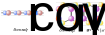
\includegraphics[width=0.5\linewidth]{img/fig-delta.pdf}
% \caption{\label{fig-delta} Scheme for the determination of the
  % covalent thickness of one-atom-thick (left) and few-atom-thick
  % (right) 2D materials.}
% \end{figure}

\begin{figure}[htbp]
\centering
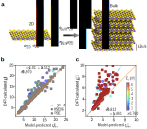
\includegraphics[width=0.75\linewidth]{./img/fig4.pdf}
\caption{\label{fig-4} \textbf{Transition of dielectric properties
    from 2D to 3D systems}. \textbf{a}. Scheme for the 2D-3D
  transition. $\alpha$ in the 2D material is essentially equivalent to
  $\varepsilon$ in its bulk counterpart. \textbf{b}
  $\varepsilon_{\mathrm{bulk}}^{\parallel}$ calculated from DFT
  (y-axis) compared with the predicted value from 2D
  $\alpha^{\parallel}$ (x-axis), showing good correlation. \textbf{c}
  $\varepsilon_{\mathrm{bulk}}^{\perp}$ calculated from DFT (y-axis)
  compared with the predicted value from 2D $\alpha^{\parallel}$
  (x-axis). The predicted value is in good aggreement with the DFT
  calculation when $E_{\mathrm{g}}>4$ eV, due to minimal interlayer
  coupling. The comparisons in \textbf{b} and \textbf{c} are made
  based on both HSE06 (circles) and PBE (squares) levels.}
\end{figure}

\begin{figure}[htbp]
  \centering
  \includegraphics[width=0.95\linewidth]{img/fig5.pdf}
  \caption{\textbf{Phase diagram of dielectric anisotropy $\eta$ as
      function of bandgap $E_{\mathrm{g}}$}. The
    $\eta$-$E_{\mathrm{g}}$ values of 2D materials (blue triangle) and
    their bulk counterparts (orange square) can be distinguished by
    the line $y=0.048x+0.087$. $\eta-E_{\mathrm{g}}$ values of
    semiconducting materials in other dimensions are also superimposed
    for comparison. Isotropic dielectric property is observed for bulk
    covalent materials (3D, red triangle) and fullerenes (0D, green
    star), while reduced dimensional materials, including planar
    organic semiconductor(OSc, 1D-2D, brown triangle), carbon nanotube
    (CNT, magenta circle) and linear OSc (0D-1D, violet pentagon) are
    scattered along the boundary line. The dimensionality and
    structure of typical materials are shown along the axis on the
    right. Compared with other materials, 2D materials and their bulk
    counterparts provide more flexibility of controlling the
    dielectric anisotropy.}
  \label{fig:aniso}
\end{figure}

\begin{figure}[htbp]
\centering
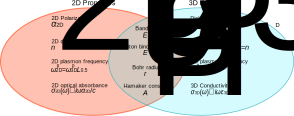
\includegraphics[width=0.75\linewidth]{img/fig-2D-vs-3D.pdf}
\caption{\label{fig-2D-3D} Dielectric-related physical quantities in
  both 2D (red circle) and 3D (cyan circle) systems. The
  dimension-dependent quantities can be related with $\alpha$ and
  $\varepsilon$, respectively. The intersection between the circles
  present the quantities are well-defined in both dimensions, but may have a
  different scaling relation with others quantities.}
\end{figure}
\end{document}